\documentclass[american,floatsintext,man]{apa6}

\usepackage{amssymb,amsmath}
\usepackage{ifxetex,ifluatex}
\usepackage{fixltx2e} % provides \textsubscript
\ifnum 0\ifxetex 1\fi\ifluatex 1\fi=0 % if pdftex
  \usepackage[T1]{fontenc}
  \usepackage[utf8]{inputenc}
\else % if luatex or xelatex
  \ifxetex
    \usepackage{mathspec}
    \usepackage{xltxtra,xunicode}
  \else
    \usepackage{fontspec}
  \fi
  \defaultfontfeatures{Mapping=tex-text,Scale=MatchLowercase}
  \newcommand{\euro}{€}
\fi
% use upquote if available, for straight quotes in verbatim environments
\IfFileExists{upquote.sty}{\usepackage{upquote}}{}
% use microtype if available
\IfFileExists{microtype.sty}{\usepackage{microtype}}{}

% Table formatting
\usepackage{longtable,booktabs}
\usepackage[counterclockwise]{rotating}   % Landscape page setup for large tables
\usepackage{multirow}		% Table styling
\usepackage{tabularx}		% Control Column width
\usepackage[flushleft]{threeparttable}	% Allows for three part tables with a specified notes section
\usepackage{threeparttablex}            % Lets threeparttable work with longtable
\usepackage{longtable}              % Allows tables to break across pages

  \usepackage{graphicx}
  \makeatletter
  \def\maxwidth{\ifdim\Gin@nat@width>\linewidth\linewidth\else\Gin@nat@width\fi}
  \def\maxheight{\ifdim\Gin@nat@height>\textheight\textheight\else\Gin@nat@height\fi}
  \makeatother
  % Scale images if necessary, so that they will not overflow the page
  % margins by default, and it is still possible to overwrite the defaults
  % using explicit options in \includegraphics[width, height, ...]{}
  \setkeys{Gin}{width=\maxwidth,height=\maxheight,keepaspectratio}
\ifxetex
  \usepackage[setpagesize=false, % page size defined by xetex
              unicode=false, % unicode breaks when used with xetex
              xetex]{hyperref}
\else
  \usepackage[unicode=true]{hyperref}
\fi
\hypersetup{breaklinks=true,
            pdfauthor={},
            pdftitle={A Quantitative Synthesis of Early Language Acquisition Using Meta-Analysis},
            colorlinks=true,
            citecolor=blue,
            urlcolor=blue,
            linkcolor=black,
            pdfborder={0 0 0}}
\urlstyle{same}  % don't use monospace font for urls

\setlength{\parindent}{0pt}
%\setlength{\parskip}{0pt plus 0pt minus 0pt}

\setlength{\emergencystretch}{3em}  % prevent overfull lines

\setcounter{secnumdepth}{0}
\ifxetex
  \usepackage{polyglossia}
  \setmainlanguage{}
\else
  \usepackage[american]{babel}
\fi

% Manuscript styling
\captionsetup{font=singlespacing,justification=justified}
\usepackage{csquotes}



\usepackage{tikz} % Variable definition to generate author note

% fix for \tightlist problem in pandoc 1.14
\providecommand{\tightlist}{%
  \setlength{\itemsep}{0pt}\setlength{\parskip}{0pt}}

% Essential manuscript parts
  \title{A Quantitative Synthesis of Early Language Acquisition Using
Meta-Analysis}

  \shorttitle{A Quantitative Synthesis}


  \author{
          Molly Lewis\textsuperscript{1},
          Mika Braginsky\textsuperscript{1},
          Sho Tsuji\textsuperscript{2},
          Christina Bergmann\textsuperscript{2},
          Page Piccinini\textsuperscript{2},
          Alejandrina Cristia\textsuperscript{2},
          Michael C. Frank\textsuperscript{1}  }

  \def\affdep{{"", "", "", "", "", "", ""}}%
  \def\affcity{{"", "", "", "", "", "", ""}}%

  \affiliation{
    \vspace{0.5cm}
          \textsuperscript{1} Department Psychology, Stanford University\\
          \textsuperscript{2} Laboratoire de Sciences Cognitives et Psycholinguistique, ENS  }


%   \def\affinst{{"init", "Department Psychology, Stanford University", "Laboratoire de Sciences Cognitives et Psycholinguistique, ENS"}}%
%   \def\affstate{{"init", "", ""}}%
%   \def\affcntry{{"init", "", ""}}%

  \note{
    \vspace{1cm}
    Author note

    \raggedright
    \setlength{\parindent}{0.4in}

    \newcounter{author}

%     %     %       %       \setcounter{author}{0}
%         %           \addtocounter{author}{1}
%         %         \expandafter\edef\csname authorid\endcsname{\theauthor}
%         Molly Lewis, \pgfmathparse{\affdep[\authorid]} \pgfmathresult, \pgfmathparse{\affinst[\authorid]} \pgfmathresult, \pgfmathparse{\affcity[\authorid]} \pgfmathresult, \pgfmathparse{\affstate[\authorid]} \pgfmathresult, \pgfmathparse{\affcntry[\authorid]} \pgfmathresult
%       %     ;
%     %       %       \setcounter{author}{0}
%         %           \addtocounter{author}{1}
%         %         \expandafter\edef\csname authorid\endcsname{\theauthor}
%         Mika Braginsky, \pgfmathparse{\affdep[\authorid]} \pgfmathresult, \pgfmathparse{\affinst[\authorid]} \pgfmathresult, \pgfmathparse{\affcity[\authorid]} \pgfmathresult, \pgfmathparse{\affstate[\authorid]} \pgfmathresult, \pgfmathparse{\affcntry[\authorid]} \pgfmathresult
%       %     ;
%     %       %       \setcounter{author}{0}
%         %           \addtocounter{author}{2}
%         %         \expandafter\edef\csname authorid\endcsname{\theauthor}
%         Sho Tsuji, \pgfmathparse{\affdep[\authorid]} \pgfmathresult, \pgfmathparse{\affinst[\authorid]} \pgfmathresult, \pgfmathparse{\affcity[\authorid]} \pgfmathresult, \pgfmathparse{\affstate[\authorid]} \pgfmathresult, \pgfmathparse{\affcntry[\authorid]} \pgfmathresult
%       %     ;
%     %       %       \setcounter{author}{0}
%         %           \addtocounter{author}{2}
%         %         \expandafter\edef\csname authorid\endcsname{\theauthor}
%         Christina Bergmann, \pgfmathparse{\affdep[\authorid]} \pgfmathresult, \pgfmathparse{\affinst[\authorid]} \pgfmathresult, \pgfmathparse{\affcity[\authorid]} \pgfmathresult, \pgfmathparse{\affstate[\authorid]} \pgfmathresult, \pgfmathparse{\affcntry[\authorid]} \pgfmathresult
%       %     ;
%     %       %       \setcounter{author}{0}
%         %           \addtocounter{author}{2}
%         %         \expandafter\edef\csname authorid\endcsname{\theauthor}
%         Page Piccinini, \pgfmathparse{\affdep[\authorid]} \pgfmathresult, \pgfmathparse{\affinst[\authorid]} \pgfmathresult, \pgfmathparse{\affcity[\authorid]} \pgfmathresult, \pgfmathparse{\affstate[\authorid]} \pgfmathresult, \pgfmathparse{\affcntry[\authorid]} \pgfmathresult
%       %     ;
%     %       %       \setcounter{author}{0}
%         %           \addtocounter{author}{2}
%         %         \expandafter\edef\csname authorid\endcsname{\theauthor}
%         Alejandrina Cristia, \pgfmathparse{\affdep[\authorid]} \pgfmathresult, \pgfmathparse{\affinst[\authorid]} \pgfmathresult, \pgfmathparse{\affcity[\authorid]} \pgfmathresult, \pgfmathparse{\affstate[\authorid]} \pgfmathresult, \pgfmathparse{\affcntry[\authorid]} \pgfmathresult
%       %     ;
%     %       %       \setcounter{author}{0}
%         %           \addtocounter{author}{1}
%         %         \expandafter\edef\csname authorid\endcsname{\theauthor}
%         Michael C. Frank, \pgfmathparse{\affdep[\authorid]} \pgfmathresult, \pgfmathparse{\affinst[\authorid]} \pgfmathresult, \pgfmathparse{\affcity[\authorid]} \pgfmathresult, \pgfmathparse{\affstate[\authorid]} \pgfmathresult, \pgfmathparse{\affcntry[\authorid]} \pgfmathresult
%       %     .
%     
    Correspondence concerning this article should be addressed to Molly
    Lewis, Psychology Department, Stanford University. 450 Serra Mall,
    Stanford, CA 94305. E-mail:
    \href{mailto:mll@stanford.edu}{\nolinkurl{mll@stanford.edu}}.

                                                                                    }

  \abstract{replicability, etc.}
  \keywords{replicability, reproducibility, meta-analysis, developmental psychology,
language acquisition \\

    \indent Word count: XXXX
  }

  \usepackage{setspace}
  \AtBeginEnvironment{tabular}{\singlespacing}
  \usepackage{pbox}

\begin{document}

\maketitle



\section{Introduction}\label{introduction}

-\textgreater{}

Psychologists hope to build generalizable theories about human
behavior---theories that hold true beyond particulars of an individual
study. The field has grown concerned as a result in the face of recent
high-profile evidence that an effect observed in one study may not be
the same in another (``replicability crisis''; Ioannidis, 2005; Nosek,
2012, 2015). Some of this variability is to be expected, however---the
question we should instead be asking is, do the data provide support for
the theory, even if they are noisy? Furthermore, to build parsimonious
theories of human behavior, we should seek to explain not just
individual phenemenon, but entire literatures of research. What is
needed, then, is a tool for aggregating noisy data across studies within
a phenomenon, as well as a common language for comparing effects across
phenomenona.

Meta-analytic methods provide a powerful tool for doing just this. The
basic unit of meta-analysis---the effect size---provides an estimate of
the \emph{size} of an effect, as well as a measure of uncertainty around
this point estimate. With such a continuous measure of success, we can
apply the same reasoning we use to aggregate noisy measurements over
participants in a single study: By assuming each \emph{study}, rather
than participant, is sampled from a population, we can appeal to the
classical statistical framework to combine estimates of the effect size
for a given phenomenon.

This quantitative approach provides a rich tool kit for synthesizing
across literatures. By describing different phenomena using the same
unit of measurement, we are able to compare effects in different
domains. Rather than simply concluding that two effects are both
``real,'' we can ask more fine-grained questions: Is effect \emph{X}
bigger than effect \emph{Y}? Does a moderator influence effect \emph{X}
in the same way as effect \emph{Y}? This type of continuous analysis
supports building quantitative models, and specifying theories that are
more precise and constraining.

In addition to these theoretical motivations, there are practical
reasons for conducting a quantitative synthesis. When planning an
experiment, an estimate of the size of an effect on the basis of prior
literature can inform the sample size needed to achieve a desired level
of power. Meta-analytic estimates of effect sizes can also aid in design
choices: If a certain paradigm tends to have overall larger effect sizes
than another, the strategic researcher might select this paradigm in
order to maximize the power of a study.

In practice, however, the feasability of this meta-analytic approach
relies on the field's commitment to practices that facilitate cumulative
science. These practices apply to all stages of the research process. At
the stage of experimental planning, researchers must pre-specify
analytical descision to limit ``researcher'' degrees of freedom
(Simmons, 2011; Simonsohn, 2014a, 2014b, 2014c). At the stage of
completion, researchers should share a result regardless of its
significance (Rosenthal, 1979; Fanelli 2012). And, at the stage of
sharing, researchers must provide enough information about the method
for another lab to conduct a close replication. Critically,r eports must
also contain complete descriptions of both data and analytical decisions
so that effect sizes can be calculcated for the purposes of
meta-analysis,

In the present paper, we use meta-analytic methods to provide a
quantitative synthesis of an entire field of psychological research:
language acquisition. We think this field is a particularly informative
case study. It may be particularly vulnerable to false findings because
running children is expensive (Ioanndis, 2005), and thus:

\begin{itemize}
\itemsep1pt\parskip0pt\parsep0pt
\item
  sample sizes are small
\item
  replications difficult and rare
\item
  Recent attention about practices in developmental research Peterson
  (2016)
\end{itemize}

We have two goals:

\begin{itemize}
\itemsep1pt\parskip0pt\parsep0pt
\item
  Describe the state of the field in terms of its participation in
  practices that are prerequisites to cumulative science, and
  ultimately, a theoretical synthesis
\item
  Provide a preliminary theoretical synthesis of the field
\end{itemize}

Towards this end, we introduce
\href{http://metalab.stanford.edu/}{Metalab}.

\section{Method}\label{method}

We analyzed 12 different phenomenena in language acquisition. We
selected these phenomena in order to describe development at many
different levels of the language hierarchy, from the acquistion of
prosody and phonemic contrasts, to gaze following in linguistic
interaction. This wide range of phenomena allowed us to compare the
course of development across different domains, as well as explore
questions about the interactive nature of language acquisition (Table
1).

To obtain estimates of effect size, we coded papers reporting
experimental data. Within each paper, we calculated a separate effect
size estimate for each experiment and age group (\enquote{conditions}).
In total, our sample includes estimates from 269 papers, 981 different
conditions and 12,029 participants. The process for selecting papers
from the literature differed by domain, with some individual
meta-analyses using more systematic approaches than others.
{[}Simulations here?{]} \renewcommand{\arraystretch}{1.5}

\begin{table}[h!]
        \footnotesize
        \begin{tabular}{lp{4cm} p{5cm}r}
            \toprule
            \textbf{Level} & \textbf{Phenomenon}                                                               & \textbf{Description}                                                                                 & \textbf{N papers (conditions)}                                                                                                                                               \\
                        \midrule

            Prosody        & IDS  preference  \newline  {\scriptsize (Dunst, Gorman, \& Hamby, 2012)}          & {\scriptsize  Looking times as a function of whether infant-directed vs. adult-directed speech is presented as stimulation.}      & 16 (50)     \\
            Sounds         & Phonotactic learning  \newline {\scriptsize (Cristia, in prep.)}                   & {\scriptsize Infants' ability to learn phonotactic generalizations from a short exposure.  }                  & 15 (47)                               \\
            ~              & Vowel discrimination (native) \newline {\scriptsize (Tsuji \& Cristia, 2014)}     & {\scriptsize Discrimination of native-language vowels, including results from a variety of methods.  }         & 40 (167)             \\ 
            ~              & Vowel discrimination (non-native) \newline {\scriptsize (Tsuji \& Cristia, 2014)} & {\scriptsize Discrimination of non-native vowels, including results from a variety of methods.  }     & 21 (72)     \\
               & Statistical sound learning  \newline {\scriptsize (Cristia, in prep.)}             & {\scriptsize Infants' ability to learn sound categories from their acoustic distribution.   }  & 11 (40) \\ 
            & Word segmentation \newline {\scriptsize  (Bergmann \& Cristia, 2015) }            & {\scriptsize Recognition of familiarized words from running, natural speech using behavioral methods.  }                     & 68 (296)                                     \\
            Words     &   Mutual exclusivity \newline {\scriptsize (Lewis \& Frank, in prep.)} &{\scriptsize  Mapping of novel words reflecting children's inference that novel words tend to refer to novel objects.}
            & 20 (60)             \\
            ~ &   Sound Symbolism \newline {\scriptsize (Lammertink et al., in prep.)} &{\scriptsize  Non-arbitrary relationship between form and meaning ("bouba-kiki effect").}
            & 10 (42)             \\
            ~              & Concept-label advantage   \newline {\scriptsize (Lewis \& Long, unpublished)}     & {\scriptsize Infants' categorization judgments in the presence and absence of labels.    } & 16 (100) \\
            ~              & Online word recognition \newline {\scriptsize (Frank, Lewis, \& MacDonald, 2016)} & {\scriptsize Online word recognition of familiar words using two-alternative forced choice preferential looking.   }              & 12 (32)                         \\
            Communication  & Gaze following  \newline {\scriptsize  (Frank, Lewis, \& MacDonald, 2016)}        & {\scriptsize Gaze following using standard multi-alternative forced-choice paradigms.   }                       & 15 (45)                                           \\
            ~              & Pointing and vocabulary  \newline {\scriptsize (Colonnesi et al., 2010)}          & {\scriptsize Longitudinal correlations between declarative pointing and later vocabulary.  }               & 25 (30)                         \\ 
            \bottomrule
        \end{tabular}
        \caption{Overview of meta-analyses in dataset.}
    \end{table}

\section{Replicability of the field}\label{replicability-of-the-field}

A literature is more likely to describe a real effect if studies are
randomly sampled from the population of all possible studies that
researchers could in principle conduct. This assumption does not mean,
however, that there should be \emph{no} variability in effect size
across studies: We should expect random variation around the true mean
effect size, with smaller studies showing more variability around this
mean.

Variability in effect sizes will be biased when this assumption of
random study sampling does not hold. Bias may be introduced by the
experimenter in a number of ways, including failure to publish null
findings (Fanelli, 2010; Rosenthal, 1979; ``publication bias'',
Rothstein, Sutton, \& Borenstein, 2006), analytical flexibility (e.g.,
``p-hacking,'' Simmons, Nelson, \& Simonsohn, 2011; Simonsohn, Nelson,
\& Simmons, 2014), reporting errors, or even fraud. These biases are
problematic for theoretical development because they lead to large but
often unknown errors in estimates of the effect size. If bias is present
in the literature, estimates of effect size may be poor estimates of the
true underlying effect size and thus be of limited evidential value. To
make theoretical progress, we must therefore distinguish variability in
effect sizes due to sample size from varability due to bias.

To assess the replicability of language acquisition phenomena, we
conducted several diagnostic analyses: Meta-analytic estimates of effect
size, fail-safe-N (Orwin, 1983), funnel plots, and p-curve (U.
Simonsohn, Nelson, \& Simmons, 2014; Simonsohn et al., 2014; Simonsohn,
Simmons, \& Nelson, 2015). These analytical approaches each have
limitations, but taken together, they provide converging evidence about
the replicability of a literature. Overall, we find little evidence of
bias in our meta-analyses, suggesting that the language acqusition
literature likely describes real psychological phenomenona and should
therefore provide the basis for theoretical development.

\subsection{Meta-analytic Effect Size}\label{meta-analytic-effect-size}

Meta-analysis provides a quantitative method for aggregating across
studies. To estimate the overall effect size of a literature, effect
sizes are pooled across papers to obtain a single meta-analytic
estimate. Importantly, meta-analysis allows us to model variability in
effect sizes due to differences in sample sizes by weighting studies
with more participants more heavily in the overall estimate. This
meta-analytic effect-size can be thought of as the ``best estimate" of
the effect size for a phenomenon given all the available data in the
literature.

Table 2, column 4 presents meta-analytic estimates for each of our
phenomenona. We find evidence for a non-zero effect size in 11 out of 12
of our phenomena, suggesting these literature provide evidential value.
In the case of phonotatic learning, however, we find that the
meta-analytic effect size estimate does not differ from zero, suggest
that this literature does not describe a real effect. {[}Remove it from
analyses below?{]}.

Meta-analytic estimates of effect size provide a categorical information
telling whether there is a real effect, or not. But, a more powerful
method of assessing evidential value would tell us the \emph{degree} to
which a literature has evidential value, and thus the degree to which it
shuold constrain our theory building. In the following three
analyses---fail-safe-N, funnel plots, and p-curves---we describe through
analyses that quantify the evidential value of these literatures.

\subsection{Fail-safe-N}\label{fail-safe-n}

One approach for quantifying the reliability of a literature is to ask,
How many missing studies with null effects would have to exist in the
\enquote{file drawer} in order for the overall effect size to be zero?
This is called the \enquote{fail-safe} number of studies (Orwin, 1983).
To answer this question, we estimated the overall effect size for each
phenomenenon (Table 2, column 2), and then used this to estimate the
fail-safe-N (Table 2, column 3).

This analysis suggests a very large number of studies would have to be
\enquote{missing} in each literature (\(M\) = 3634) in order for the
overall effect sizes to be 0. Thus, while it is possible that some
reporting bias is present in the literature, the large fail-safe-N
suggests that the literature nonetheless likely describes a real effect.

One limitation of this analysis, however, is that it assumes that all
reported effect sizes are obtained in the absence of analytical
flexibility: If experimenters are exercising analytical flexibility
through practices like p-hacking, then then number and magnitude of
observed true effects in the literature may be inflated. In the next
analysis, we examine this possibility through funnel plots.

\subsection{Funnel Plots}\label{funnel-plots}

Funnel plots provide a visual method for evaluating whether variability
in effect sizes is due only to differences in sample size. A funnel plot
shows effect sizes versus a metric of sample size, standard error. If
there is no bias in a literature, we should expect studies to be
randomly sampled around the mean, with more variability for less precise
studies.

Figure 1 presents funnel plots for each of our 12 meta-analyses. These
plots show evidence of asymmetry (bias) for several of our phenomenon
(Table 2, column 4). However, an important limitation of this method is
that it is difficult to determine the source of this bias. One
possibility is that this bias is due not to experimenter, but to true
heterogenity in phenomena (e.g.~different ages). P-curve analyses
provide one method for addressing this issue, which we turn to next.

\begin{figure}[htbp]
\centering
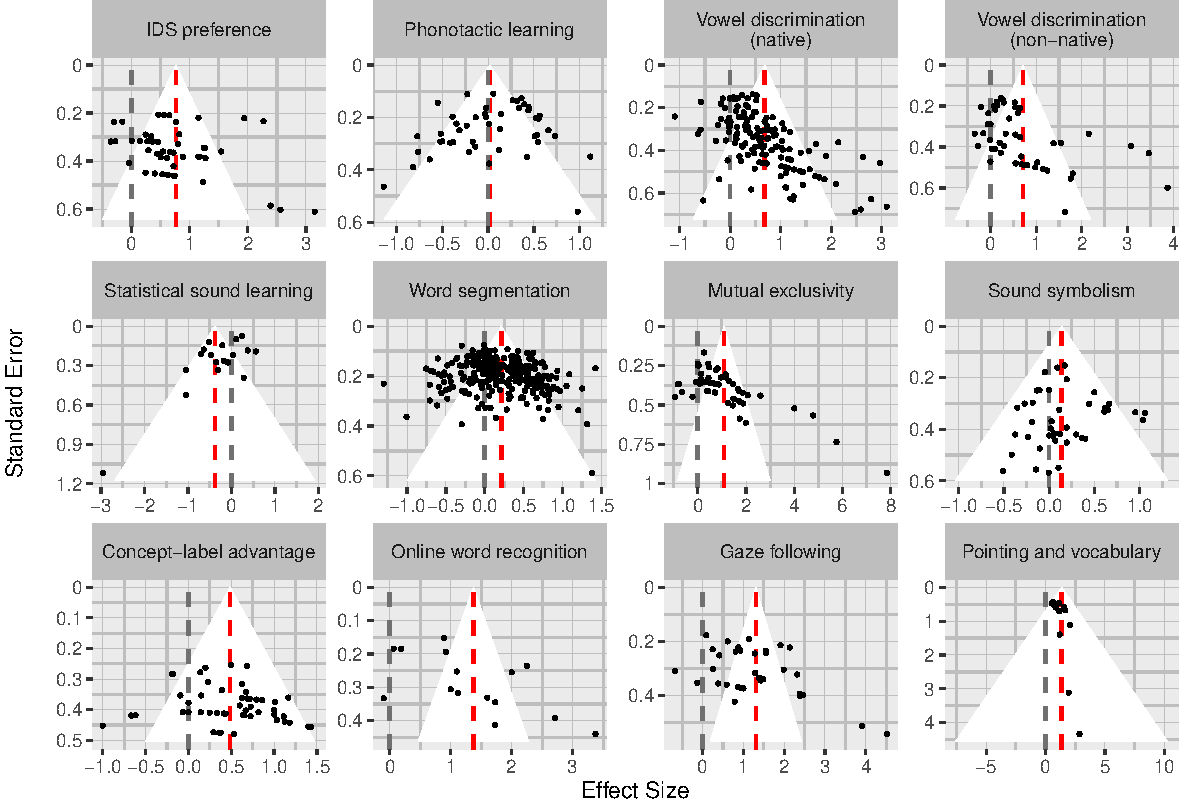
\includegraphics{metalab_synthesis_files/figure-latex/unnamed-chunk-2-1.pdf}
\caption{Funnel plots for each meta-analysis. Each effect size estimate
is represented by a point, and the mean effect size is shown as a red
dashed line. The funnel corresponds to a 95\% (narrow) and 99\% (wide)
CI around this mean. In the absense of true heterogenity in effect sizes
(no moderators) and bias, we should expect all points to fall inside the
funnel.}
\end{figure}

\subsection{P-curves}\label{p-curves}

\begin{figure}[htbp]
\centering
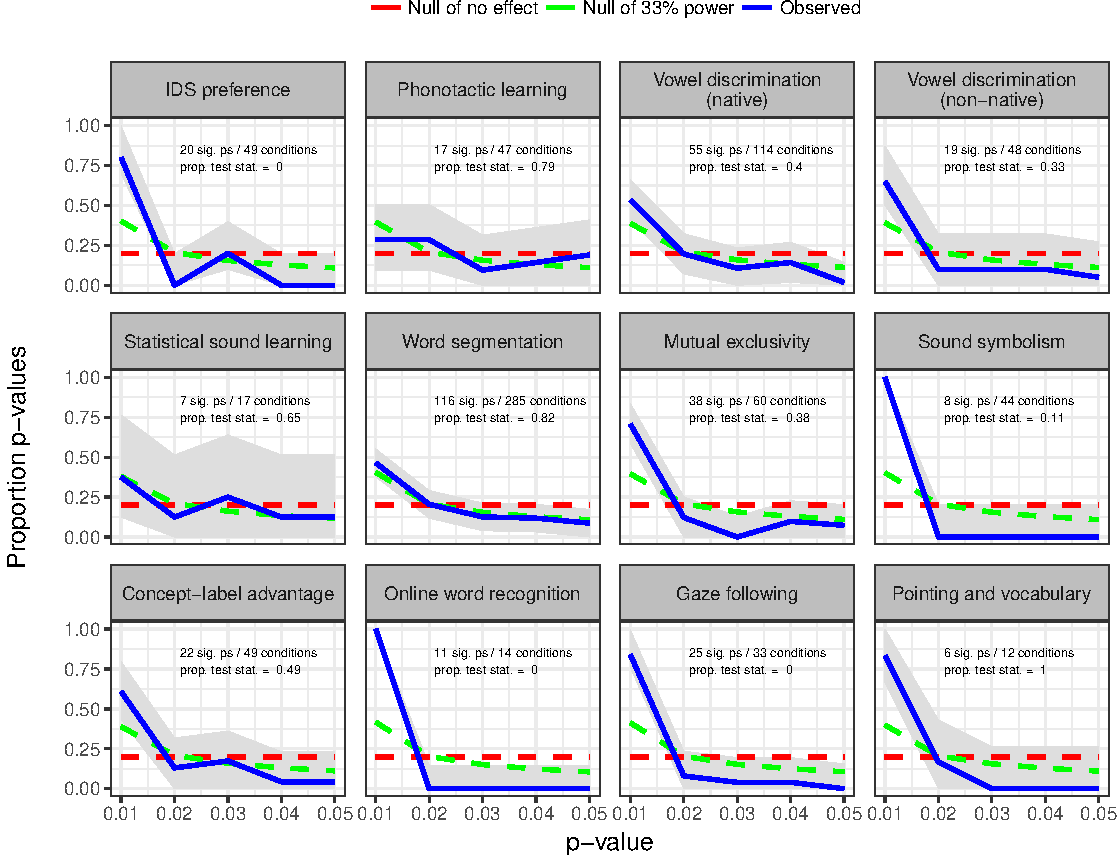
\includegraphics{metalab_synthesis_files/figure-latex/p_curve_plots-1.pdf}
\caption{P-curve for each meta-analysis (Simonsohn, Nelson, \& Simmons,
2014). In the absense of p-hacking, we should expect the observed
p-curve (blue) to be right-skewed (more small values). The red dashed
line shows the expected distribution of p-values when the effect is
non-existent (the null is true). The green dashed line shows the
expected distribution if the effect is real, but studies only have 33\%
power.}
\end{figure}

P-curves provide a more robust way to identify bias in a literature (U.
Simonsohn et al., 2014; Simonsohn et al., 2014, 2015). A p-curve is the
distribution of p-values for the statistical test of the main hypothesis
across a literature. Critically, if there is a real effect in the
literature, the shape of the p-curve should reflect this. In particular,
we should expect the p-curve to be right skewed with more small values
(e.g., .01) than large values (e.g., .04). An important features of this
method is that we should expect this skew independent of any true
heterogenity in the data, such as age. Evidence that the curve is in
fact right-skewed would suggest that the literature is not biased, and
that it provides evidential value for theory building.

\begin{table}[t]
\footnotesize
\begin{tabular}{lrrrrr}
\toprule
\textbf{Phenomenon}& \textbf{\textit{d}} & \textbf{fail-safe-N} & \textbf{funnel skew} & \textbf{p-curve skew} & \textbf{power}\\
\midrule
IDS preference & 0.71 [0.53, 0.89] & 3762 & 1.88 (0.06) &  & \\
Phonotactic learning & 0.04 [-0.09, 0.16] & 45 & -1.08 (0.28) & -1.52 (0.06) & 0.14\\
Vowel discrimination (native) & 0.6 [0.5, 0.71] & 9536 & 8.98 (0) & -5.42 (0) & 0.67\\
Vowel discrimination (non-native) & 0.66 [0.42, 0.9] & 3391 & 4.13 (0) & -3.24 (0) & 0.78\\
Statistical sound learning & -0.14 [-0.27, -0.02] & Inf & -1.87 (0.06) &  & \\
Word segmentation & 0.2 [0.15, 0.25] & 5645 & 1.54 (0.12) & -9.67 (0) & 0.56\\
Mutual exclusivity & 1.01 [0.68, 1.33] & 6443 & 6.25 (0) &  & \\
Sound symbolism & 0.15 [0.04, 0.26] & 538 & -1.32 (0.19) & -2.16 (0.02) & 0.96\\
Concept-label advantage & 0.4 [0.29, 0.51] & 3928 & 0.31 (0.76) & -6.15 (0) & 0.69\\
Online word recognition & 1.89 [0.81, 2.96] & 2843 & 2.92 (0) &  & \\
Gaze following & 0.84 [0.26, 1.42] & 2641 & -1.69 (0.09) &  & \\
Pointing and vocabulary & 0.41 [0.32, 0.49] & 1202 & 0.59 (0.55) &  & \\
\bottomrule
\end{tabular}
\caption{Summary of replicability analyses. \textit{d} = Effect size (Cohen's {\it d}) estimated from a random-effect model; fail-safe-N = number of missing studies that would have to exist in order for the overall effect size to be {\it d} = 0; funnel skew = test of asymmetry in funnel plot using the random-effect Egger's test (Stern \& Eggers, 2005); p-curve skew = test of the right skew of the p-curve using the Stouffer method (Simonsohn, Simmons, \& Nelson, 2015); power = power to reject the null hypothesis at the 5\% significance level based on the p-curve (Simonsohn, Nelson, \& Simmons, 2014);  Brackets give 95\% confidence intervals, and parentheses show p-values.}
\end{table}

Figure 2 shows p-curves for 7 of our 12
meta-analyses\footnote{We were unable to do this analysis on all meta-analyses because some were missing key statistical tests (e.g. gaze following) or the test statistic was not available (e.g. pointing and vocabulary).}.
Across all p-curves, the curves show evidence of right skew. This is
confirmed by formal analyses (Table 2, column 5). P-curves also provide
a method for calculcating the overall power of a literature, based on
the shape of the p-curve (U. Simonsohn et al., 2014). Intuitively, when
power is high and effect is real, we should be more likely to observe an
effect size \enquote{further} from the null. This means that we will
observe more small effect sizes. Thus, the higher the power, the more
right skewed the p-curve will be. Table 2 (column 6) presents estimates
of power for each meta-analysis based on p-curve. With the exception of
phonotactic learning (\emph{power} = 0.14), literatures appear to have
acceptable power.

\section{Theoretical Synthesis}\label{theoretical-synthesis}

Given this literature has evidential value, we next turn to drawing
inferences on the basis of the literature.

\subsection{Statistical Approach}\label{statistical-approach}

METAMETAPLOT

\section{Discussion}\label{discussion}

Limitations

\paragraph{Author Contributions}\label{author-contributions}

\paragraph{Acknowledgments}\label{acknowledgments}

\newpage

\subsubsection{References}\label{references}

\setlength{\parindent}{-0.5in} \setlength{\leftskip}{0.5in}
\setlength{\parskip}{8pt}

Bergmann, C., \& Cristia, A. (2015). Development of infants'
segmentation of words from native speech: A meta-analytic approach.
\emph{Developmental Science}.

Dunst, C., Gorman, E., \& Hamby, D. (2012). Preference for
infant-directed speech in preverbal young children. \emph{Center for
Early Literacy Learning}, \emph{5}(1).

Fanelli, D. (2010). Positive Results Increase Down the Hierarchy of the
Sciences. \emph{PLoS ONE}, \emph{5}(4), e10068--10.

Frank, M. C., Lewis, M. L., \& MacDonald, K. (in press). A performance
model for early word learning. In \emph{Proceedings of the 38th Annual
Conference of the Cognitive Science Society}. Retrieved from
\url{http://langcog.stanford.edu/papers_new/frank-2016-underrev.pdf}

Lewis, M., \& Frank, M. C. (in prep). Multiple routes to disambiguation.

Orwin, R. G. (1983). A fail-safe n for effect size in meta-analysis.
\emph{Journal of Educational Statistics}, 157--159.

Peterson, D. (2016). The Baby Factory: Difficult Research Objects,
Disciplinary Standards, and the Production of Statistical Significance.
\emph{Socius: Sociological Research for a Dynamic World}, \emph{2}(0),
1--10.

Rosenthal, R. (1979). The file drawer problem and tolerance for null
results. \emph{Psychological Bulletin}, \emph{86}(3), 638.

Rothstein, H. R., Sutton, A. J., \& Borenstein, M. (2006).
\emph{Publication bias in meta-analysis: Prevention, assessment and
adjustments}. John Wiley \&amp; Sons.

Simmons, Nelson, L. D., \& Simonsohn, U. (2011). False-Positive
Psychology: Undisclosed Flexibility in Data Collection and Analysis
Allows Presenting Anything as Significant. \emph{Psychological Science},
\emph{22}(11), 1359--1366.

Simonsohn, U., Nelson, L. D., \& Simmons, J. P. (2014). P-curve and
effect size correcting for publication bias using only significant
results. \emph{Perspectives on Psychological Science}, \emph{9}(6),
666--681.

Simonsohn, Nelson, L. D., \& Simmons, J. P. (2014). P-curve: A key to
the file-drawer. \emph{Journal of Experimental Psychology: General},
\emph{143}(2), 534.

Simonsohn, Simmons, J. P., \& Nelson, L. D. (2015). Better p-curves.
\emph{Simonsohn, Uri, Joseph P. Simmons, and Leif D. Nelson
(Forthcoming),``Better P-Curves,'' Journal of Experimental Psychology:
General}.

Sterne, J. A., \& Egger, M. (2005). Regression methods to detect
publication and other bias in meta-analysis. \emph{Publication Bias in
Meta-Analysis: Prevention, Assessment, and Adjustments}, 99--110.

Tsuji, S., \& Cristia, A. (2014). Perceptual attunement in vowels: A
meta-analysis. \emph{Developmental Psychobiology}, \emph{56}(2),
179--191.



\end{document}
